%
% Este archivo es parte de un documento sobre OpenERP/Odoo creado
% y distribuido bajo licencia GNU Free Documen License v1.3.
%
% Para obtener la fuente e información más detallada, visite
% https://github.com/Gabriel-fm/oerp-manual
%
% Copyright (c) 2014 - Gabriel Franco
%


\chapter{Módulo de Almacén}
\label{moduloAlmacen}
El stock es la parte física de sus productos, cosas más que datos. Por ello, necesitan ser almacenados y trasladados entre ubicaciones, y hacer un seguimiento en grupos e individualmente. Tienen un tamaño, un peso y un coste. OpenERP gestiona todo este de una manera única y práctica.

La gestión del stock por OpenERP es muy simple, flexible y completa. Se basa en el concepto de la doble entrada que \emph{revolucionó} la contabilidad. El sistema puede ser descrito por la máxima de Lavoisier “nada perdido, todo cambiado” o, mejor, “todo  se movió”. En OpenERP no se habla de desaparecer, consumir o perdida de productos: en su lugar se habla sólo de movimientos de stock de un lugar a otro.


Al igual que en contabilidad, OpenERP gestiona contrapartidas para cada una de sus operaciones como recibos de proveedores, envío a clientes, beneficio y perdidas de inventario y consumo de materiales. Los movimientos de stock siempre se hacen de una ubicación a otro. Para satisfacer esta necesidad de una contrapartida para cada movimiento de stock, el software permite distintos tipos de ubicación para el stock.

\begin{itemize}
\item Ubicaciones físicas del stock
\item Ubicaciones de cliente
\item Ubicaciones virtuales como contrapartida para la producción e inventario
\end{itemize}

Las ubicaciones físicas representan almacenes físicos y su estructura jerárquica. Estos son generalmente las ubicaciones que son manejadas por los sistemas de stock tradicionales.

Las ubicaciones de los clientes representan los stocks de sus clientes y proveedores. Para seguir con la analogía de contabilidad, estos almacenas representan el papel de las cuentas de terceros. Recibir de un proveedor puede mostrarse como un movimiento de bienes de una ubicación de otra empresa a una ubicación física en su propia compañía. Como ve, las ubicaciones de proveedor muestran normalmente un stock negativo y las ubicaciones de cliente tendran un stock positivo.


Las ubicaciones virtuales como contrapartida para la producción, son utilizadas en las operaciones de manufactura. Manufacturar se caracteriza por el consumo de materiales y la producción de productos finales. Las ubicaciones virtuales se usan como contrapartida de estas dos operaciones. En el caso que nos concierne, no trataremos con ellas.


Las ubicaciones del inventario son contrapartidas de las operaciones del stock, representando los beneficios y perdidas de su compañía en términos de stock.

En OpenERP, las ubicaciones se estructuran jerárquicamente. Puede estructurar sus ubicaciones como un árbol o con relaciones padre-hijo. Esto brinda niveles más detallados de análisis de sus operaciones de stock y de la organización de su almacén.

En OpenERP un Almacén representa el lugar donde su stock físico se encuentra almacenado. Un Almacén puede estructurarse en varias ubicaciones y multiples niveles. Las ubicaciones se usan para gestionar todo tipo de lugares de almacenamiento, tal como las contrapartidas del cliente y producción.



\section{Conceptos en gestión de stock}
Para mostrar el concepto de gestión de stock veremos como se generan los movimientos de stock a través de las siguientes operaciones:

\begin{itemize}
\item Recibir productos de un proveedor
\item Envíos a clientes
\item Operaciones de inventario para materiales perdidos
\end{itemize}

Estos movimientos se muestran en tablas para hacerlo visualmente más comprensible:

\begin{table}[!th]
\begin{center}
\begin{tabular}{|c|c|}
  \hline
  Ubicación & Productos \\
  \hline
  Ubicaciones $>$ Proveedores & -30 bicicletas \\
  \hline
  Ubicaciones físicas $>$ Su empresa $>$ Stock & +30 bicicletas \\
  \hline
  
\end{tabular}
\end{center}
\caption{Compra de stock}
\label{al:compra}
\end{table}

En la tabla \ref{al:compra} se observa como al obtener stock, se muestra la aparición del mismo en las instalaciones de la empresa, mientras que aparece la cantidad equivalente, pero en negativo, en las ubicaciones del proveedor. Esto muestra como el proveedor se deshace de dos bicicletas mientras que en nuestro almacén aparecen dos bicicletas. El resultado de la operación, si todo está correcto y el stock se mueve de forma correcta es que todo suma siempre cero. 

De forma equivalente a esto, se realizan los movimientos de stock hacia los clientes como se muestra en la tabla \ref{al:venta} a continuación

\begin{table}[!th]
  \begin{center}
  \begin{tabular}{|c|c|}
    \hline
    Ubicación & Poductos \\
    \hline
    Ubicaciones físicas $>$ Su compañia $>$ Stock & -2 bicicletas \\
    \hline
    Ubicaciones clientes $>$ Clientes europeos & +2 biciletas \\
    \hline
  \end{tabular}
  \end{center}
  \caption{Venta de stock}
  \label{al:venta}

\end{table}

Así puede ver que la suma de stocks de un producto en todas las ubicaciones de OpenERP es siempre cero. En contabilidad se diría que la suma de débitos es igual a la suma de créditos.

Las ubicaciones de las empresas (de clientes y proveedores) no se localizan jerárquicamente bajo su empresa, así pues sus contenidos no se consideran parte de su stock. Así que si mira en la ubicación física dentro de su compañía, esas dos bicicletas no están más en su compañía. Aunque no se encuentren en su stock físico, es todavía muy útil el verlos en el stock de su cliente, ya que ayudará a llevar un análisis de la gestión de stock detallada.

En la gestión del stock, es complicado evitar un salto entre los datos en el software y las cantidades reales en el stock. La gestión de doble entrada del stock da el doble de oportunidades para encontrar un error. Si olvida dos items del stock, este error se reflejará automáticamente en la ubicación de la contrapartida.


Puede realizar una comparación con contabilidad, ya que podrá encontrar errores fácilmente ya que puede buscar errores en las cuentas propias o en las contrapartidas: si no hay suficiente en la cuenta del banco es, probablemente, porque alguien olvidó introducir el pago de una factura de cliente. Sabe que siempre la suma de debitos debe ser igual a la suma de créditos tanto en contabilidad como en la gestión de stock de OpenERP.
En contabilidad, todos los documentos apuntan a entradas de contabilidad que forman la base de la gestión contable. Si crea facturas, por ejemplo, los resultados de las operaciones son entradas de contabilidad en las cuentas. Y de igual forma para la gestión del stock en OpenERP. Todas las operaciones de stock se llevan a cabo como movimientos de stock. Ya si empaqueta productos o los manufactura o realiza una operación sobre el inventario en el stock, los movimientos de stock lo reflejarán en todo momento.


Se ha visto un ejemplo simple de recepción de bienes y envío de productos, pero algunas operaciones son menos obvias – una operación de inventario en el stock, por ejemplo. Una operación de inventario se lleva a cabo cuando se compara el stock mostrado en el software con los productos reales contados en los almacenes.

En OpenERP, con su gestión de doble entrada de stock, debería usar los movimientos de stock para estas operaciones de inventario. Esto ayudará a la trazabilidad del stock. Suponga que hay 26 bicicletas en el stock real, pero OpenERP muestra 28 en el sistema. Debe pues, reducir el número en OpenERP a 26. Esta reducción de 2 unidades se considera una perdida o destrucción de productos y la corrección se realiza con la siguiente operación:

\begin{table}[!th]
\begin{center}
\begin{tabular}{|c|c|}
  \hline
  Ubicación & Productos \\
  \hline
  Ubicaciones físicas $>$ Su empresa $>$ Stock & -2 bicicletas \\
  \hline
  Ubicaciones virtuales $>$ Perdidas de inventario & +2 bicicletas \\
  \hline
\end{tabular}
\end{center}
\caption{Operación de ajuste de stock}
\label{al:perdidas}
\end{table}

Después de unos meses, usted puede realizar evaluaciones del stock en la ubicación a través de Control de Inventario $>$ Estructura de ubicaciones $>$ ubicaciones virtuales $>$ Perdidas de inventario. Esto le dará el valor de perdidas de stock de la compañía en un periodo dado.

Una vez comprendido como funciona la gestión de stock en OpenERP, se puede pasar al analisis de cada elemento del módulo de Almacén.


\section{Recepción/Envios por Pedidos}
En esta parte del módulo de gestión de almacén se lleva el control del movimiento de stock desde y hacia la compañia. Se entiende cada uno de los movimientos en esta sección como un albarán en el que se engloba, como un único pedido, varios productos.

La creación de estos albaranes puede ser tanto manual como automática. La creación automática de estos albaranes viene en consecuencia de la creación de ordenes de venta a clientes y pedidos de compra a proveedores. Estas acciones, aparte del movimiento económico que conllevan, implican un cambio en el stock de la empresa, tanto una minimización del mismo en las ventas como un engrosamiento en el caso de compras. También existen albaranes de movimientos de stock internos en el caso de que la compañia mantenga varias ubicaciones físicas de stock, controlando en cualquier caso qué y cuánto material hay en cada sitio.

En el caso de las ventas, cuando alguién en la sección ventas lleva a cabo el proceso comercial con éxito, resultando en la facturación al cliente, con la aprobación de la venta se generará a su par un albarán de salida en el que estarán reflejados los productos que han sido vendidos en esa transacción, a qué cliente se envían y el resto de datos relacionados con el proceso. De esta manera, el encargado de almacén, tan sólo tiene que estar atento a esta, su sección, para saber que materiales deben salir del almacén y a que dirección han de ser enviados. De igual manera, al realizar una compra, el encargado sabrá que ha de haber una recepción de material, especificando cuál y cuánto, para poder confirmar que la compra se ha realziado con éxito.



\subsection{Albaranes de entrada}
\subsubsection{LISTADO DE ALBARANES}

\begin{figure}[H]
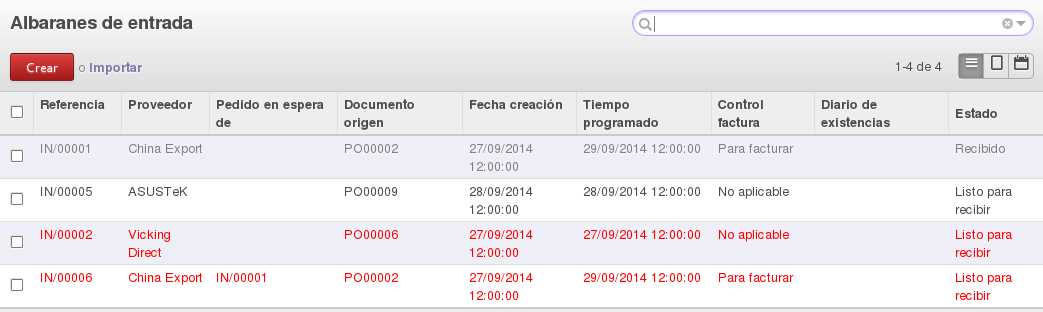
\includegraphics[width=\textwidth]{almacen/img/alb_entrada.png}
\caption{Albaranes de entrada}
\end{figure}

Al entrar en la sección de albaranes de entrada, se ofrecerá una visión general de todos los albaranes para los pedidos entrantes en sus distintos estados. En una visión general, los distintos campos representados serán:

\begin{description}
  \item[Referencia] 
    Una referencia a este albarán/pedido. Usado para control interno. 
  \item[Proveedor] 
    Proveedor del que se espera la recepción de material.
  \item[Pedido en espera de]
    Este campo es usado en caso de que se realicen recepciones parciales de material. Si cuando se espera un pedido, se recibe sólo una parte del mismo, al indicar que parte de material se recibe, se crea un segundo albarán que contendrá el resto de materiales a recibir, indicando en este campo de que albarán original depende ese material a recibir.
  \item[Documento origen] 
    Cuando se realizan los pedidos desde las ordenes de compra u otros lugares, este campo hace referencia a ese documento que originó la recepción de material. En el caso del ejemplo se puede ver que los albarances tienen como documento de origen pedidos de compra.
  \item[Fecha de creación] 
    Fecha en la que se creó el albarán.
  \item[Tiempo programado] 
    Fecha en la que se espera la recepción del producto. Para el cálculo de la misma se tiene en cuenta los datos ya introducidos en el proveedor y en los productos, en los que se puede indicar los tiempos de espera que suelen tener ese proveedor/producto.
  \item[Control factura] 
    Especifica el estado de facturación del pedido. Este campo también dependerá de como se haya generado el pedido. Hay pedidos que pueden facturarse una vez recibidos y habrá pedidos que se facturen antes de ser recibidos. En la captura del ejemplo se puede observar como una de las recepciones está lista para facturar, mientras que el resto la factura es a priori.
  \item[Diario de existencias] 
    En este campo se especifica si el albarán/pedido es parte de algún diario de existencias. Estos \emph{diarios} sirven para aglutinar distintos albaranes bajo la responsabilidad del dueño del diario. Si existen responsables distintos para la recepción de diferentes productos, se puede especificar en este campo. 

Esto es útil a efectos de análisis de responsabilidades en el caso de tener diferentes responsables de materiales en almacén. También puede utilizarse para indicar quién es el encargado de la recepción de ese pedido en el momento de llegada. Usarlo de una u otra manera queda en función de como gestione la empresa el almacen.
  \item[Estado] 
    Estado del albarán. Este puede variar entre distintos estados. Los habituales en este caso son \emph{Recibido} y \emph{Listo para recibir}.
\end{description}

\vspace{0.5cm}


\subsubsection{Vista de un albarán}

En la lista anterior, al hacer click sobre alguna linea de albarán, se pasará a la vista de un albarán y sus contenidos, de manera más especifica que la visión en la lista. En este punto se detallará el contenido esperado del pedido y más especificaciones.

\begin{figure}[H]
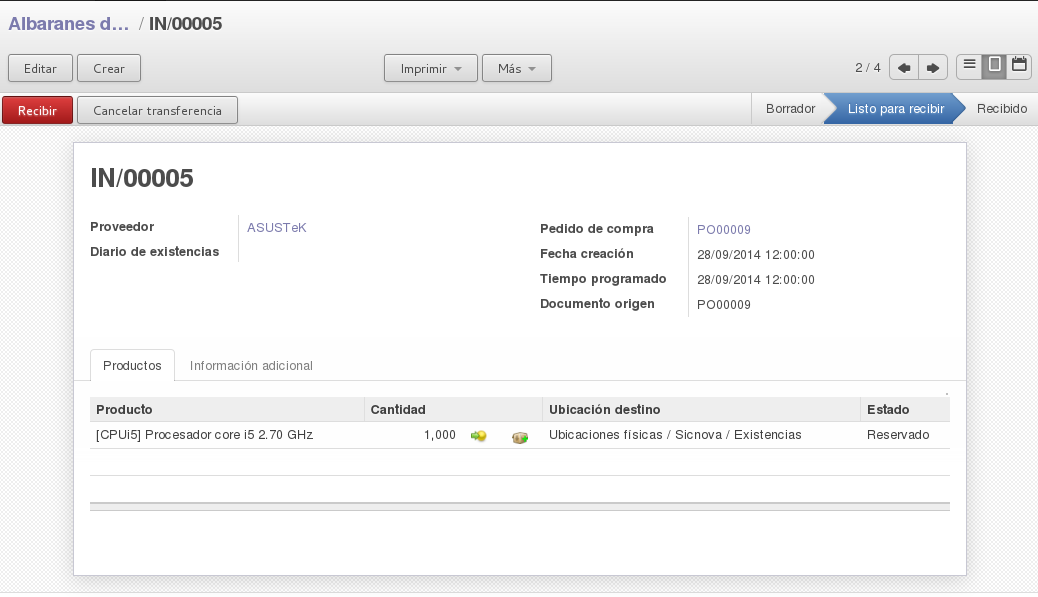
\includegraphics[width=\textwidth]{almacen/img/alb_entrada_i.png}
\caption{Albarán de entrada individual}
\end{figure}

En la parte superior del albarán individual se pueden observar los campos que se veían cuando se abría la lista de albaranes de entrada.

En la parte inferior se pueden observar dos pestañas. La primera de ellas es \textbf{Productos}. En esta pestaña se listarán los productos que se esperan de ese pedido. En cada una de las lineas se especificará uno de los productos a recibir y los elementos de cada línea se componen de los siguientes elementos:

\begin{description}
  \item[Producto] Se especfica el nombre del producto y su referencia según se ha especificado al crear el producto.

  \item[Cantidad] Indica el número de productos de ese tipo a recibir en la recepción de este albarán.

  \item[Botón de deshechar productos] Con este botón se pueden pasar productos de la recepción a una ubicación virtual denominada \emph{Productos deshechados} que indicarían que tales productos no han sido validos y han sido deshechados.

Con esta acción se abrirá una nueva ventana emergente en la que se preguntará que cantidad de producto es la que va a ser deshechada y permitirá indicar en que ubicación de almacén de deshecho se registrará el movimiento de stock (en caso de que haya varias)

  \item[Botón Poner en un nuevo paquete] Permite indicar que cierta parte del pedido de ese producto en concreto llegará o ha llegado en un nuevo paquete.

Al seleccionar esta opción se abrirá una ventana emergente en la que se preguntará que cantidad del producto elegido \textbf{se quedará} en el albarán actual.

  \item[Ubicación destino] Este campo describe en que ubicación del almacén será el que albergue los productos una vez sean recibidos.

  \item[Estado] Indica, en ese producto, cuál es su estado en el stock. Esto quiere decir que ese producto que se va a recibir puede tener alguno de los siguientes estados:

    \begin{description}
    \item[Reservado] \hfill \\ Cuando los productos a recibir están reservados quiere decir que existe otro movimiento (normalmente una venta) que está a la espera de recibir stock de ese producto para poder ser realizado
    \item[Esperando disponibilidad] \hfill \\ Si el producto está en este estado es que simplemente está a la espera de la recepción del paquete. Una vez que el paquete se recibe se supone que este producto está disponible. En este caso el producto no se encuentra reservado ni pedido por otra transacción de almacén.
    \end{description}
\end{description}

\vspace{0.5cm}

La pestaña \textbf{Información adicional} contiene algunos datos extra sobre la recepción del pedido, algunos de los cuales pueden ser modificados por el responsable de almacén si se da el caso.

\begin{figure}[H]
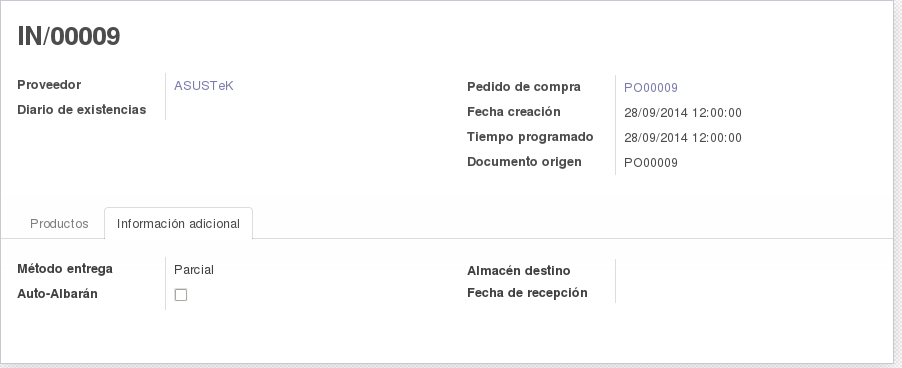
\includegraphics[width=\textwidth]{almacen/img/alb_entrada_m.png}
\caption{Pestaña de información adicional}
\end{figure}


\begin{description}
  \item[Método de entrega] Puede ser \textbf{Parcial} si se puede recibir en varias partes los distintos productos, o \textbf{Todo junto} si la recepción se realiza en un solo paquete.
  \item[Auto-Albarán] Esta opción es creada cuando se utiliza OpenERP para la manufactura de productos. Añade un elemento más de control sobre los productos que son la base de la manufactura de otros.

Esto quiere decir que, cuando existe una orden de creación de un producto, si faltan los elementos base, se generará un pedido de los mismos y cuando estos productos base lleguen, si la opción Auto-albarán \textbf{está} activada, estos elementos base pasarán directamente al proceso de manufactura. En el caso de que \textbf{no} se encuentre seleccionada, habrá que dar un paso extra y antes de realizar la manufactura, dar el visto bueno al uso y movimiento de esos productos base.
  \item[Almacén destino] Almacén en el que se guardará el producto.
  \item[Fecha recepción] Fecha en la que se ha recibido el paquete.
\end{description}

\vspace{0.5cm}

\subsubsection{Estados del albarán}
Con esto, se conoce ya el contenido y funcionamiento de los albaranes de entrada. Sólo queda aclarar sus posibles estados. Los estados posibles para los albaranes de entrada son los que se pueden ver en la parte superior derecha de la pantalla cuando se está visualizando un albarán individual.

\begin{itemize}
\item[$\star$] \textbf{Borrador} -- Cuando se crea un albarán desde la misma pantalla del albarán mediante el botón \emph{Crear} en la parte superior de la pantalla, pasará a estar en este estado. Es, como su propio nombre indica, un estado aún no confirmado y que puede continuar editandose. En este estado, los pasos posibles (realizables por los botones situados en la parte superior de la pantalla) son:
  \begin{itemize}
  \item[--] \textbf{Confirmar} - Confirma el borrador y lo pasa al estado \emph{Listo para recibir}
  \item[--] \textbf{Confirmar y recibir} - Confirma el borrador y pasa directamente a confirmar la recepción de los productos mediante un dialogo en el que se especifica cuantos productos de los especificados en el albarán han llegado. Esto hace que, si todos los productos son recibidos, el albarán pase directamente a \textbf{Recibido}
  \item[--] \textbf{Cancelar transferencia} - Con esto se cancela el albarán y todos los calculos relativos a cambios en el stock. Si se cancela no se podrá volver a utilizar, teniendo que crear uno nuevo dado el caso.
  \end{itemize}


\item[$\star$] \textbf{Listo para recibir} -- Este estado indica que el borrador ha sido confirmado. Cuando el albarán se crea desde una orden de compra (y en general, cuando es creado automáticamente) este es su estado por defecto. Desde este estado el albarán puede utilizar los botones de estado siguientes:
  \begin{itemize}
  \item[--] \textbf{Recibir} - Presentará el dialogo de confirmación del número de productos recibidos para confirmar su inclusión en el stock. Tras esto, el albarán pasará a su estado de \emph{Recibido}. En el caso de que no todos los productos hayan sido recibidos, se generará automáticamente otro albarán en estado \textbf{Listo para recibir} que contendrá como productos los no incluidos en la recepción del albarán original.
  \item[--] \textbf{Cancelar transferencia} - Se cancela el albarán y todos los calculos relativos a cambios en el stock. Si se cancela no se podrá volver a utilizar, teniendo que crear uno nuevo dado el caso.
  \end{itemize}
  

\item[$\star$] \textbf{Recibido} -- Cuando el producto ha sido recibido el albarán pasará a este estado.
  \begin{itemize}
  \item[--] \textbf{Crear factura/abono} - Esta opción estará disponible sólo si el producto fué configurado de manera que el pago del mismo se haga en la recepción.
  \item[--] \textbf{Devolver productos} - Usado en caso de que sea necesario realizar alguna devolución. Esta opción abrirá una ventana de dialogo en la que se especificará la cantidad de que producto será devuelta y si la devolución \textbf{será abonada por parte del proveedor o no}.

Esta devolución creará automáticamente un albarán de salida con los datos del proveedor y los productos indicados en esta devolución.

El dialogo de devolución de productos se puede ver en la figura \ref{al:devolver}
  \end{itemize}
\end{itemize}


\begin{figure}[H]
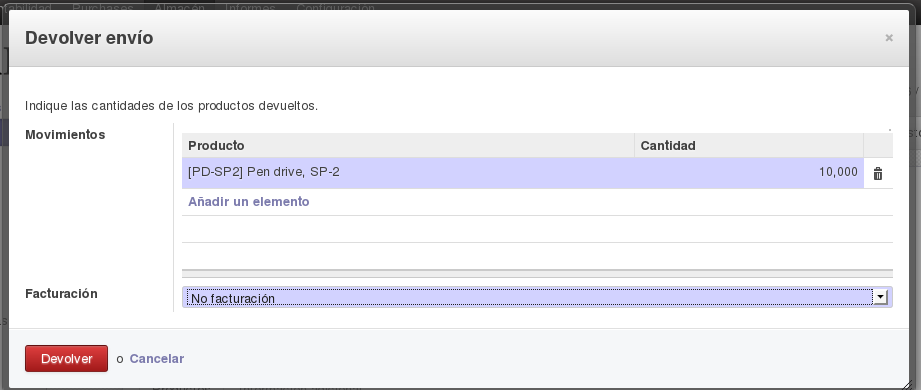
\includegraphics[width=\textwidth]{almacen/img/alb_entrada_dev.png}
\caption{Pestaña de devolución de productos}
\label{al:devolver}
\end{figure}




\vspace{0.5cm}
\subsection{Albaranes internos}
Los albaranes internos son utilizados en el caso de que su empresa tenga dos o más ubicaciones donde almacenar sus productos. En tales casos estos albaranes informan de cambios de ubicación entre las instalaciones de la empresa.


\vspace{0.5cm}
\subsection{Albaranes de salida}
Los albaranes de salida son los que hacen referencia a movimientos de productos desde un almacén propiedad de su empresa y los clientes. Se entienden como movimientos de salida de stock. La creación de los mismos se puede realizar de forma manual o de forma automática a través del modulo de ventas, generando una orden de venta.

En su concepción más básica, los albaranes de salida son y funcionan prácticamente igual que los albaranes de entrada. A continuación se va a recalcar principalmente las diferencias entre los albaranes de entrada y salida, pasando rápidamente por las secciones iguales y equivalentes en ambos tipos de albaranes.

\subsubsection{LISTADO DE ALBARANES DE SALIDA}
\label{almacen:envio}

\begin{figure}[H]
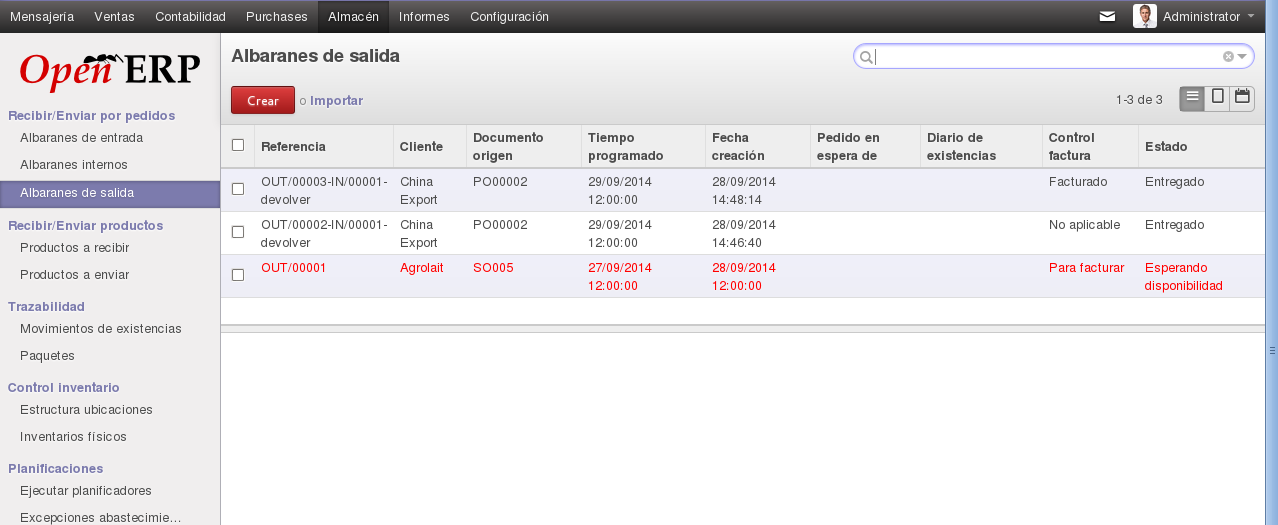
\includegraphics[width=\textwidth]{almacen/img/alb_salida.png}
\caption{Listado de albaranes de salida}
\label{al:listasalida}
\end{figure}

Los campos que se pueden observar en el listado de albaranes de salida son:

\begin{description}
  \item[Referencia] -- Referencia del albarán. Permite ver de un vistazo si es un albarán de salida normal o corresponde a alguna variación como a una devolución (pueden observarse dos albaranes de devolución en la figura \ref{al:listasalida}

  \item[Cliente] -- Cliente al que hace referencia el albarán y al que se le entregarán los productos.

  \item[Documento origen] -- Si el albarán ha sido generado automáticamente, este campo apunta al documento que dió lugar a su creación.

  \item[Tiempo programado] -- Tiempo calculado para servir los productos.

  \item[Fecha creación] -- Fecha en la que se ha creado el albarán

  \item[Pedido en espera de] -- Equivalente al mismo campo en los albaranes de entrada. Cuando se realiza un envío, puede realizarse por partes por las razones que sean (falta de stock, paquetes distintos) Cuando se realiza de tal manera, los productos del albarán que \textbf{no} son enviados, son incluidos en un nuevo albarán de salida, y ese albarán de salida tendrá este campo apuntando a ese albarán original con los materiales enviados.

  \item[Diario de existencias] -- Equivalente al mismo campo en los albaranes de salida.
 
  \item[Control factura] -- Al igual que en los albaranes de entrada, indica el estado de facturación, si procede, del albarán.

  \item[Estado] -- Indica el estado de los productos. Las posibilidades son:
    \begin{itemize}
    \item[*] \textbf{Borrador} -- Un albarán no confirmado y a la espera de ser confirmado o borrado.
    \item[*] \textbf{Esperando disponibilidad} -- Se encuentra a la espera de que los productos del albarán se encuentren disponibles.
    \item[*] \textbf{Lista para envío} -- Los productos están disponibles y es posible realizar el envío.
    \item[*] \textbf{Entregado} -- El albarán ha sido procesado integramente
    \end{itemize}
\end{description}


\vspace{0.5cm}
\subsubsection{ALBARAN DE SALIDA INDIVIDUAL}
Al igual que en los albaranes de entrada, hacer click sobre uno de los albaranes lo abrirá de manera individual mostrando los detalles del mismo.

\begin{figure}[H]
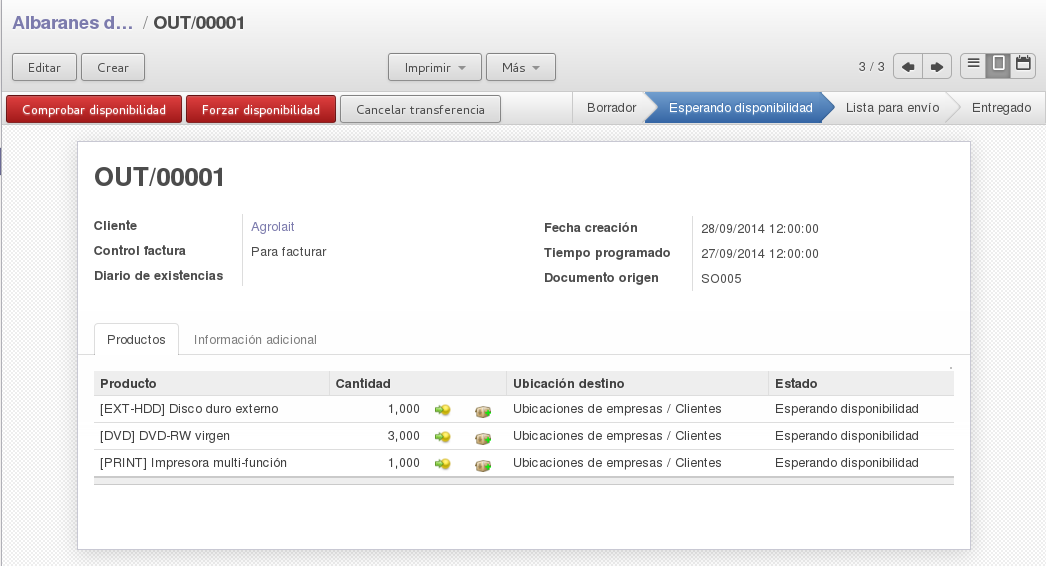
\includegraphics[width=\textwidth]{almacen/img/alb_salida_i.png}
\caption{Albarán de salida individual}
\label{al:salidaind}
\end{figure}

La parte superior del albarán es, al igual que en los albaranes de entrada, los mismos datos que se ven cuando se visualiza la lista de todos los albaranes de salida.

En la parte inferior están las mismas dos pestañas que en los albaranes de entrada con un funcionamiento idéntico. En este punto, la diferencia principal está en los posibles estados de cada producto. En este caso, los posibles estados son:

\begin{description}
  \item[Nuevo] -- Cuando se crea el albarán a mano y no ha sido confirmado aún.
  
  \item[Esperando otro movimiento] -- En caso de que el producto deba pasar por algún movimiento previo, el producto estára en este estado.

  \item[Esperando disponibilidad] -- En este caso, no hay suficiente disponibilidad del producto y queda a la espera de las variaciones del inventario hasta ser favorable.

  \item[Disponible] -- Existe stock del producto y puede ser enviado.

  \item[Reservado] -- Cuando se comprueba la disponibilidad de los productos mediante el botón homónimo en la parte superior del albarán, si existe suficiente stock del producto, lo reservará. Esto quiere decir que si se reserva en un albarán y aparece otro albarán después que requiere de los mismos productos, este segundo albarán verá el stock de productos como el total de los disponibles \textbf{menos} los reservados, evitando así que pedidos que no tienen material reservado se adelanten a otros que ya están siendo preparados.

En el caso de estar reservados y que por cualquier razón tengan que eliminar tal reserva, para ello se ha de hacer click sobre la línea del producto reservado y en la ventana emergente del producto (figura \ref{al:prodreser}, utilizar el botón \textbf{Cancelar disponibilidad}
\end{description}

\begin{figure}[H]
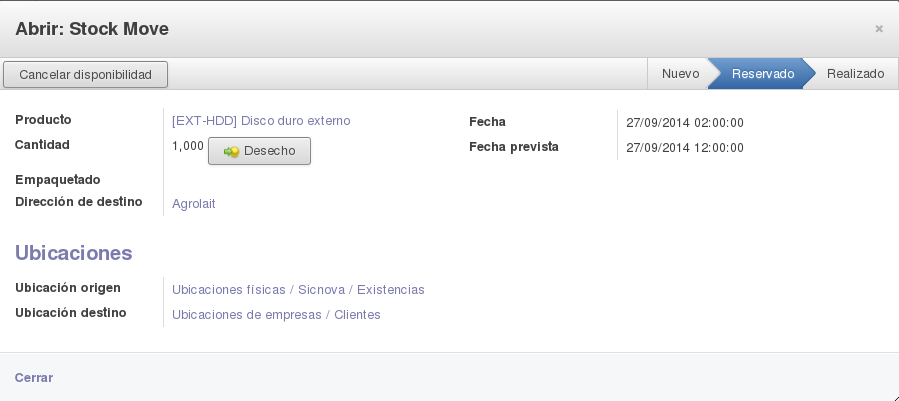
\includegraphics[width=\textwidth]{almacen/img/alb_salida_res.png}
\caption{Línea de un producto reservado para salida}
\label{al:prodreser}
\end{figure}

\vspace{0.5cm}
\subsubsection{ESTADOS DEL ALBARAN}

Los distintos estados y transiciones en los albaranes de salida son:

\begin{itemize}

  \item[$\star$] \textbf{Borrador} -- Albarán por confirmar, aún editable en todos sus campos. Este estado se da por defecto cuando se crea el albarán a través del botón \emph{Crear}.

    \begin{itemize}
      \item[--] \textbf{Confirmar} - Confirma el albarán y le permite pasar al estado \emph{Esperando disponibilidad}.
      \item[--] \textbf{Confirmar y enviar} - Confirma el albarán y da por enviados los productos. Da dos pasos en un solo click.
      \item[--] \textbf{Cancelar} - Cancela el albarán. Este paso no permite volver a ponerlo en estado de disponibilidad, hay que volver a crearlo tras cancelarlo.
    \end{itemize}



  \item[$\star$] \textbf{Esperando disponibilidad} -- Cuando el borrador es confirmado o cuando el albarán es creado automáticamente desde una orden de venta, pasará a este estado. En este punto pueden ocurrir dos cosas según si existe stock o no de alguno de los productos de las líneas.

    \begin{itemize}
    \item[--] \textbf{Existe stock de alguna línea de producto} - Si en algún producto hay stock, el albarán pasará al estado de \emph{Lista para el envío} en el caso de que la opción \emph{Método de entrega} de la pestaña \emph{Información adicional} tenga su valor en \emph{Parcial}. 

En caso de que su valor sea \emph{Todo junto}, sólo pasará al estado \emph{Lista para envío} cuando todos los productos estén disponibles.
      
    \item[--] \textbf{No existe stock de ningún producto} - En tal caso se permite la elección entre tres posibles pasos
      \begin{itemize}
      \item \textbf{Comprobar disponibilidad} Realiza un chequeo del stock de los productos. Si existe stock suficiente de alguna de las líneas de productos, realizará la reserva de los mismos y según el valor de \emph{Método de entrega} (explicado en el punto anterior) podrá pasar al estado de \emph{Lista para el envío}.

      \item \textbf{Forzar disponibilidad} Fuerza los productos como disponibles, situando el stock de los mismos en números negativos si es necesario y pasando el albarán al estado de \emph{Lista para el envío}.
      \end{itemize}
    \end{itemize}




  \item[$\star$] \textbf{Lista para envío} -- En este estado alguno o todos los productos se encuentran disponibles para el envío. En este punto sólo pueden realizarse dos acciones:

    \begin{itemize}
    \item[--] \textbf{Enviar} - Da por enviados los productos y realiza los cambios en el stock.
    \item[--] \textbf{Canclear} - Cancela el albarán y la transferencia de productos.
    \end{itemize}
\end{itemize}






\vspace{0.5cm}
\section{Recibir/Enviar Productos}
Los datos a los que se pueden acceder a través de las secciones de este menú son los mismos que en los submenús de la sección \emph{Recibir/Enviar por pedidos} con la salvedad de que se presentan de forma distinta.

En la sección anterior los datos se agrupaban por albaranes. Cada pedido/venta estaba relacionado con un albarán, el cual podía contener varías lineas de productos. En la actual sección se van a representar esas líneas de producto de forma independiente a los albaranes. Esto quiere decir que esta vista nos va a permitir ver los productos que están por entrar o por salir independientemente de sus albaranes y de los productos que puedan acompañarles en los mismos.

\subsection{Productos a recibir}
Las líneas representadas en esta sección corresponde a todos los productos contenidos en los albaranes de entrada.

\subsubsection{LISTADO DE PRODUCTOS A RECIBIR}

La vista por defecto al entrar en esta sección es la de la figura \ref{al:prodentrada}

\begin{figure}[H]
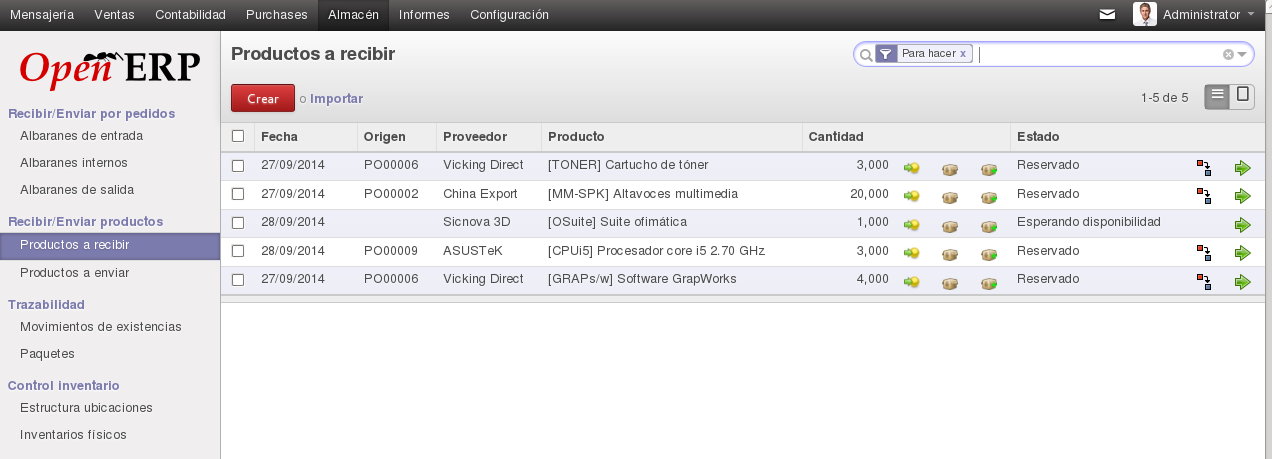
\includegraphics[width=\textwidth]{almacen/img/prod_entrada.png}
\caption{Lista de productos entrantes}
\label{al:prodentrada}
\end{figure}

Los campos disponibles son similares a los que se han visto en secciones anteriores relacionadas con los albaranes. En un repaso rápido y una explicación de algunos nuevos botones:

\begin{itemize}
  \item[*]\textbf{Fecha} -- Fecha de creación de la línea de pedido
  \item[*]\textbf{Origen} -- Documento que ha generado esta línea de pedido (si existe)
  \item[*]\textbf{Proveedor} -- Proveedor del producto
  \item[*]\textbf{Producto} -- Producto de la línea de pedido
  \item[*]\textbf{Cantidad} -- Cantidad de productos a recibir
  \item[*]\textbf{Botón de deshechar} -- No se utiliza desde los productos a recibir con la configuración actual. Es útil en caso de que en la recepción se utilizarán diversas ubicaciones físicas para la recepción del material y por el camino pudiera deshecharse parte del mismo.
  \item[*]\textbf{Botón de poner en el paquete actual} -- 
  \item[*]\textbf{Botón poner en un nuevo paquete} -- Realiza la división de los productos en varios paquetes.

Por defecto, cuando se piden X unidades de un producto, todas aparecen en la misma línea, representando esto que vienen en el mismo paquete. Mediante este botón se puede dividir el número de unidades de un producto en varias líneas, representando con esto que venían divididos en varios paquetes.

  \item[*]\textbf{Estado} -- Estado del pedido del producto. Más adelante se explica cuales son y como varían sus estados.

  \item[*]\textbf{Botón de procesado parcial} -- Cuando el producto se encuentra reservado, pueden procesarse parte de ese pedido para que forme parte del stock.

  \item[*]\textbf{Botón Realizado} -- Hacer click sobre este botón va a procesar esa línea del producto y va a dar por recibido ese producto incorporandolo al stock.

\end{itemize}


\subsubsection{LINEA DE PEDIDO INDIVIDUAL}

Al hacer click sobre uno de los elementos en el listado, se abrirá una visión individual del mismo como se ve en la figura \ref{al:prodentradai}

\begin{figure}[H]
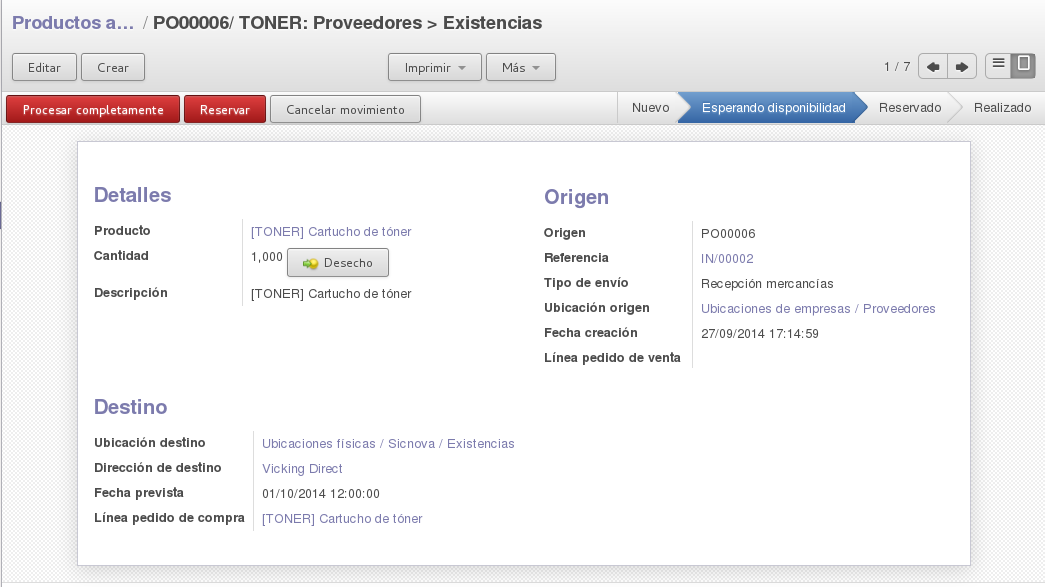
\includegraphics[width=\textwidth]{almacen/img/prod_entrada_i.png}
\caption{Linea de entrada individual}
\label{al:prodentradai}
\end{figure}

La visión individual engloba tres áreas con distinta información como son:

\begin{description}
  \item[Detalles] -- Que especifican los datos del producto de esa línea
    \begin{itemize}
    \item[$\star$] \textbf{Producto} - Nombre del producto que enlaza a la ficha del mismo
    \item[$\star$] \textbf{Cantidad} - Número de unidades del producto esperadas
    \item[$\star$] \textbf{Descripción} - Descripción del producto, insertada en la creación del mismo.
    \end{itemize}


  \item[Destino] -- Contiene la información relativa al lugar al que se va a realizar el movimiento de stock.
    \begin{itemize}
      \item[$\star$] \textbf{Ubicación destino} - Ubicación donde se contabilizará el stock
      \item[$\star$] \textbf{Dirección de destino} - Una desafortunada traducción. En este campo se indica la dirección y ficha de datos del proveedor.
      \item[$\star$] \textbf{Fecha prevista} - Fecha prevista de recepción de los productos.
      \item[$\star$] \textbf{Línea pedido de compra} - Nombre de la línea en el albarán.
    \end{itemize}

  \item[Origen] - Información relativa al origen de pedido, de la línea y del producto.
    \begin{itemize}
      \item[$\star$] \textbf{Origen} - Documento que origina el albarán en el que se encuentra la línea de producto.
      \item[$\star$] \textbf{Referencia} - Enlace al albarán que ha generado esta línea de producto
      \item[$\star$] \textbf{Tipo de envío} - Especifica que tipo de envío es, pudiendo elegirse entre \emph{Recepción de mercancías}, \emph{Envío de mercancías} e \emph{Interno}.
      Esta opción se rellena automáticamente según que tipo de albarán haya genereado esa línea de producto, sólo hay que rellenarla manualmente si se crean líneas de pedido individuales desde esta sección.
      \item[$\star$] \textbf{Ubicación origen} - Ubicación origen de la que aparecen estos productos.
      \item[$\star$] \textbf{Fecha creación} - Fecha en la que se ha creado la línea de pedido
      
    \end{itemize}
\end{description}

\vspace{.5cm}
Cuando la línea está creada correctamente y su estado es \textbf{Esperando disponibilidad} (ha pasado del su estado \emph{Nuevo} a \emph{Esperando disponibilidad} en el caso de crearla manualmente) pueden darse tres pasos con esa línea tal y como se ve en la figura \ref{al:prodentradai} anterior.
\begin{itemize}
\item[*] \textbf{Procesar completamente} - Da por recibidos los productos y pasa esta línea al estado de \textbf{Realizado}
\item[*] \textbf{Reservar} - Realiza la reserva en el stock de los productos, reflejandolo en las ubicaciones del stock e influyendo en lineas de pedidos posteriores, que tendrán en cuenta si hay más o menos stock según las reservas.
\item[*] \textbf{Cancelar movimientos} - Cancela estas líneas en el albarán correspondiente
\end{itemize}

\vspace{.5cm}
Cuando se realiza la reserva se pasa la línea al estado de \textbf{Reservado}. En este estado sólo caben dos opciones, tres si tenemos en cuenta que se pueden recibir productos parcialmente, los botones en ese estado se pueden ver en la figura \ref{al:prodentradares}

\begin{figure}[H]
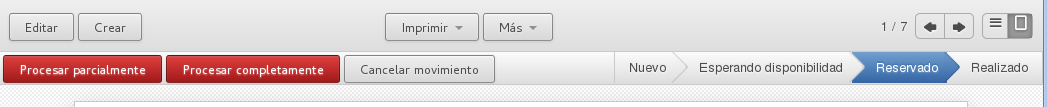
\includegraphics[width=\textwidth]{almacen/img/prod_salida_state.png}
\caption{Botones en el estado ``Reservado''}
\label{al:prodentradares}
\end{figure}

\begin{itemize}
\item[*] \textbf{Procesar parcialmente} - Mostrará un diálogo con el que se permite procesar sólo una parte de todo el pedido. Se usa cuando llega sólo una cantidad de productos que no es la esperada por la línea de producto.
\item[*] \textbf{Procesar completamente} - Da por recibido todos los productos y pasa la línea al estado de \textbf{Realizado}
\item[*] \textbf{Cancelar movimiento} - Cancela la línea de pedido.
\end{itemize}

\subsection{Productos a enviar}
En esta parte, el funcionamiento y la presentación de la información de las líneas es exactamente igual que en la anterior. 

La diferencia principal es que, en este caso, las líneas que se muestran son las de los productos de los \textbf{albaranes de salida}. Esto quiere decir que es una especie de sección espejo, se maneja y fucniona igual que \emph{Productos a recibir} con la salvedad de que hay que tener en cuenta que los movimientos de stock van \emph{al revés}.

Si en la sección anterior se podían ver y manipular los productos que venían de los proveedores al stock de nuestra empresa, en esta sección hay que tener claro que se está trabajando con movimientos que van desde nuestro stock hacia los clientes.






\section{Trazabilidad}

\subsection{Movimientos de existencias}
Esta sección muestra \textbf{todos} los movimientos de productos línea a línea, tanto los envíados como los recibidos. Da una visión global de todos
los movimientos para busquedas avanzadas.

También se incluyen aquí movimientos que no están relacionados directamente con los albaranes como pueden ser las ordenes de abastecimiento creadas
por las cantidades mínimas de stock como se verá más adelante.

\begin{figure}[H]
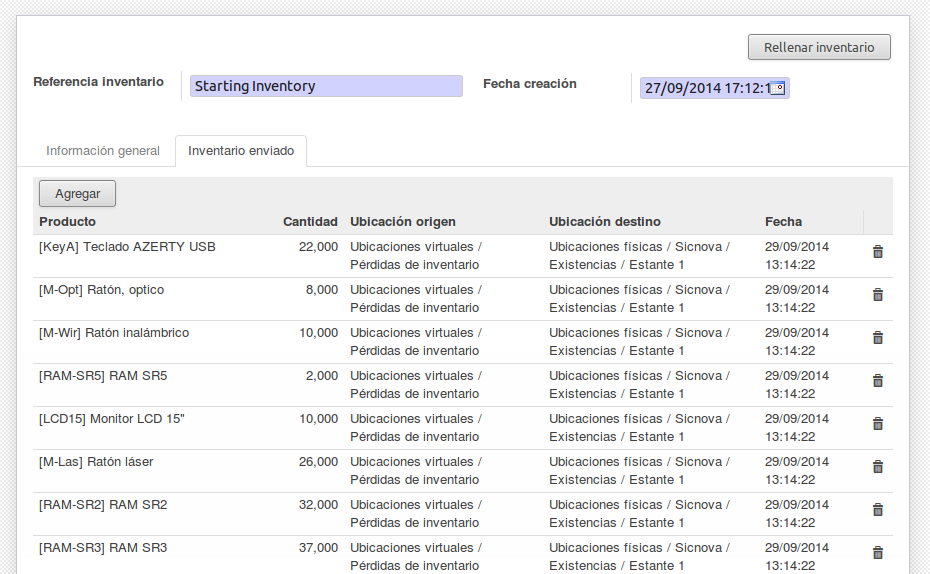
\includegraphics[width=\textwidth]{almacen/img/tra_mov.png}
\caption{Pantalla de movimiento de existencias}
\label{al:movex}
\end{figure}

%\subsection{Paquetes}






\section{Control Inventario}

A través de esta sección se llevará el inventario y se podrá controlar de forma semiautomática los inventarios y movimientos, así como las posibles perdidas de inventario y otros detalles relativos al stock.

\subsection{Estructura ubicaciones}
Aquí se va a presentar un menú desplegable y una zona para desplegar información en forma de árbol.

El desplegable permite elegir entre los tres tipos de ubicaciones posibles:
\begin{description}
  \item[Ubicaciones físicas] -- Ubicaciones que representan un espacio físico concreto como puede ser las zonas de almacenaje de las empresas. Se representa en la figura \ref{ub:fisicas}
\begin{figure}[H]
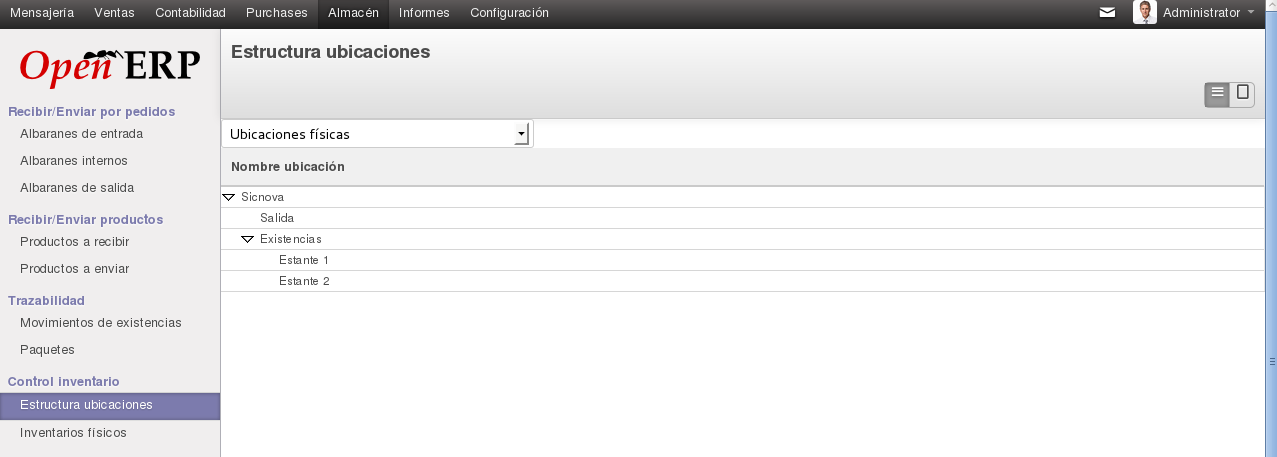
\includegraphics[width=\textwidth]{almacen/img/ubi_fisica.png}
\caption{Ejemplo de ubicaciones físicas}
\label{ub:fisicas}
\end{figure}

  \item[Ubicaciones de empresas] -- Ubicaciones relativas a clientes, proveedores y envíos internos.
  \item[Ubicaciones virtuales] -- Este tipo de ubicaciones es también importante ya que entre ellas se puede encontrar la ubicación de \emph{Pérdidas de inventario} que puede ser crítica para el análisis del stock. Puede verse en la figura \ref{ub:virtuales}
\end{description}


\begin{figure}[H]
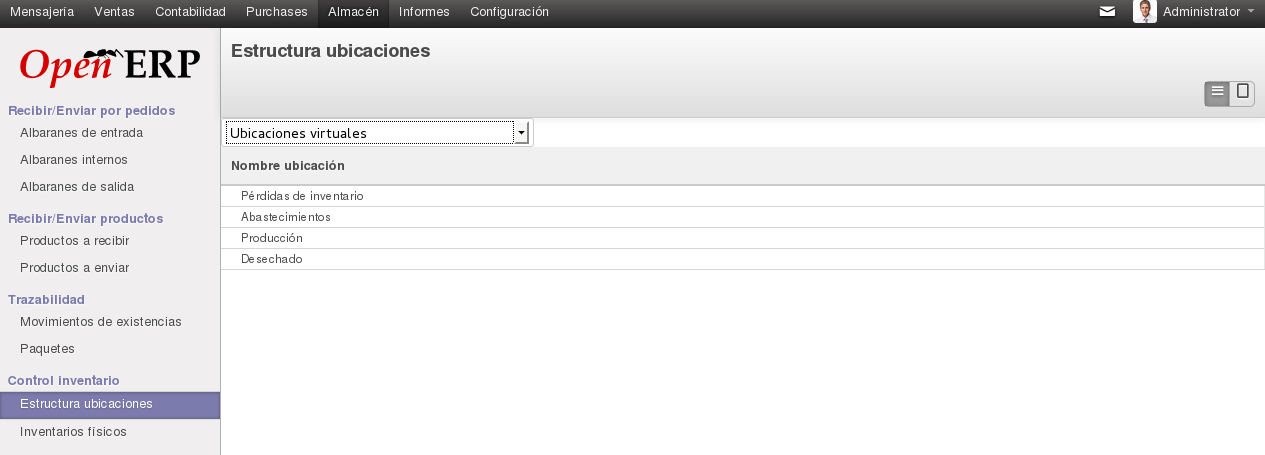
\includegraphics[width=\textwidth]{almacen/img/ubi_virtual.png}
\caption{Ubicaciones virtuales por defecto}
\label{ub:virtuales}
\end{figure}


Hacer click sobre cualquiera de estas ubicaciones abrirá un diálogo que llevará a una visualización del inventario en la ubicación marcada. Este dialogo permitirá elegir como mostrar el inventario mediante la elección del \emph{Tipo de análisis}. El menú es el que se puede ver en la figura \ref{ub:inventariomenu}. Las opciones de esta elección son:


\begin{itemize}
  \item \textbf{Analizar inventorio actual} - Muestra el inventorio teniendo en cuenta \emph{todos} los movimientos de stock
                                            en la base de datos
  \item \textbf{Analizar periodo} - Permite elegir la fecha inicial y final para el análisis del inventario. Es lo más
                                   práctico para análisis más minuciosos.
\end{itemize}

\begin{figure}[H]
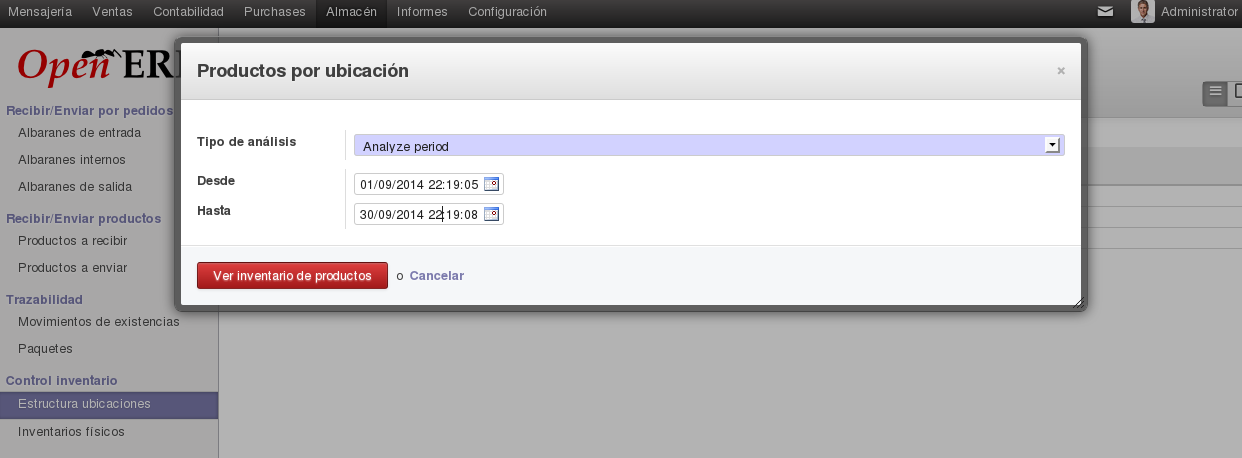
\includegraphics[width=\textwidth]{almacen/img/ubi_invent_menu.png}
\caption{Menú de análisis de inventario}
\label{ub:inventariomenu}
\end{figure}


El inventario mostrado contiene la información de los productos existentes en el mismo y una previsión de los que habrá cuando se vayan aprobando los distintos albaranes y transacciones de productos. Un ejemplo de este inventario se puede ver en la figura \ref{ub:inventarioej} con una descripción de los campos tras la figura.

\begin{figure}[H]
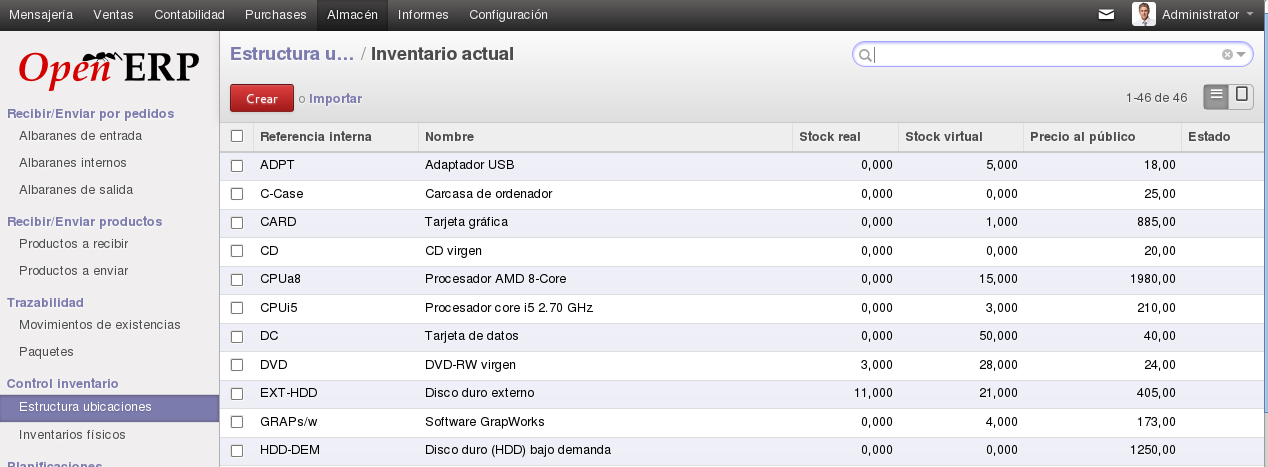
\includegraphics[width=\textwidth]{almacen/img/ubi_inventario.png}
\caption{Inventario físico de ejemplo}
\label{ub:inventarioej}
\end{figure}


\begin{description}
  \item[Referencia interna] -- Referencia del producto. Especificada en la ficha del mismo.
  \item[Nombre] -- Nombre del producto.
  \item[Stock real] -- Stock existente en el momento actual.
  \item[Stock virtual] -- Stock que pasará a ser real en cuanto se ejecuten las transacciones de productos pendientes. Este stock se calcula mediante
                          el stock real - stock saliente + stock entrante, siendo estos dos últimos (entrante y saliente) las operaciones pendientes
  \item[Precio al público] -- Precio del producto al público. Especificado en la ficha del producto.
\end{description}


\subsection{Inventarios físicos}
Los inventarios físicos, como su nombre indica, hacen referencia a los inventarios, los recuentos de material disonibles físicamente. En esta zona del
programa es a través de la cual se informará de los recuentos de material y se mezclará con la información de las transacciones de productos realizadas
para finalmente poder obtener un informe detallado de lo que se tiene y de lo que se debería tener y, por ende, fallos en transacciones, en recuentos, 
existencia de material perdido...

\subsubsection{Listado de inventarios}
Al entrar en esta opción, la primera visión de los inventarios es un listado de los mismos (figura \ref{ub:inventariolista}). Los datos visibles de los mismos serán:

\begin{itemize}
  \item \textbf{Referencia inventario} -- Referencia del inventario que se le da a la hora de crearlo.
  \item \textbf{Fecha de creación} -- Fecha en la que se ha creado el inventario.
  \item \textbf{Estado} -- Estado del inventario. El mismo puede tener tres estados:
    \begin{itemize}
      \item[$\star$] \textbf{Borrador} - Se han hecho los recuentos apropiados pero no se ha confirmado. En este estado, la información contenida
                                         en el inventario no modifica la información de stock de los productos en la base de datos.
      \item[$\star$] \textbf{Confirmado} - El paso siguiente tras el borrador. En este estado, la información de recuentos se refleja en la base de
                                           datos. En este caso, los recuentos influyen sólo en el stock virtual.
      \item[$\star$] \textbf{Realizado} - Una vez confirmado y comprobados todos los pasos, se valida el inventario. Es en este momento en el que
                                          los calculos pasan a ser efectivos y se modifica el stock real en la base de datos.
    \end{itemize}
\end{itemize}

\begin{figure}[H]
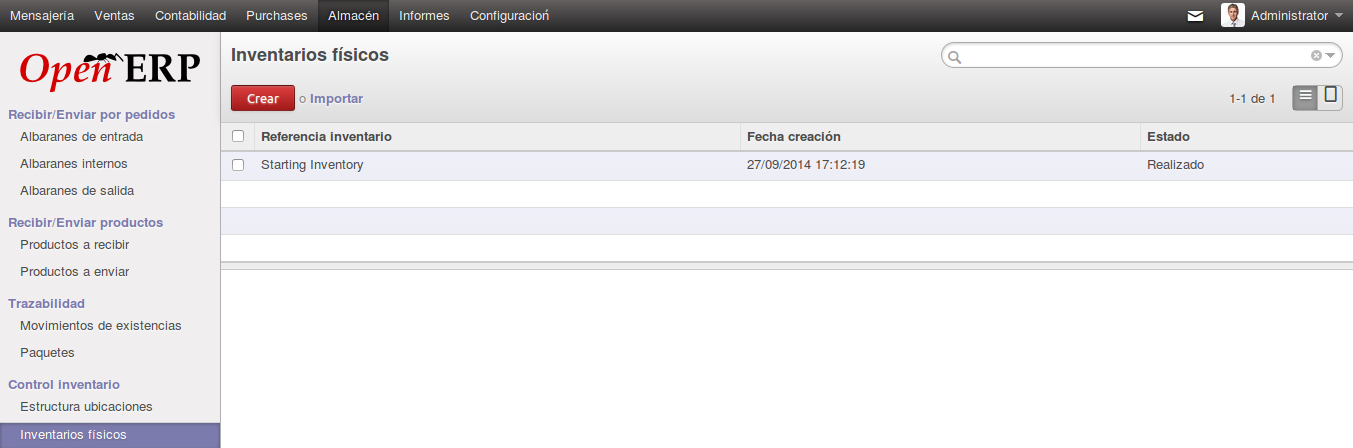
\includegraphics[width=\textwidth]{almacen/img/inv_lista.png}
\caption{Listado de inventarios}
\label{ub:inventariolista}
\end{figure}	

Haciendo click sobre uno de los inventarios o pulsando el botón de crear, se procede al inventario seleccionado o a crear un nuevo inventario como se
ve en la figura \ref{ub:inventarioindividual}. Los datos a rellenar son los mismos que los que se han visto en el listado de inventarios aparte de dos
pestañas que se rellenan con los datos del inventario.

En la pestaña de \textbf{información general} (también se puede ver en la figura \ref{ub:inventarioindividual}) los datos a rellenar son:

\begin{itemize}
  \item \textbf{Ubicación} -- Ubicación física en la que se encuentra el material recontado.
  \item \textbf{Producto} -- Producto que se está inventariando.
  \item \textbf{Cantidad} -- Cantidad de producto a inventariar.
\end{itemize}

\begin{figure}[H]
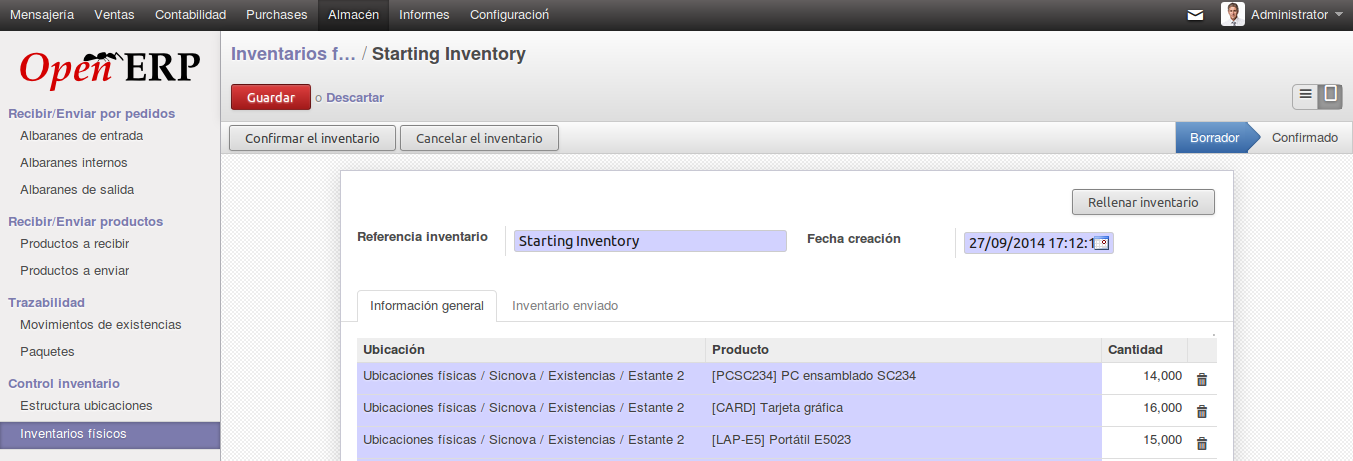
\includegraphics[width=\textwidth]{almacen/img/inv_ind.png}
\caption{Edición de inventario}
\label{ub:inventarioindividual}
\end{figure}	

El botón \emph{Rellenar inventario} ayuda a importar el inventario actual. Abre una ventana emergente (figura \ref{ub:inventarioimportar}) que,
una vez seleccionada la ubicación, importa todos los productos contenidos en esa ubicación y su número actual en la lista de productos del inventario
que se está creando/rellenando. La importación admite dos opciones que se presentan como checkboxes:

\begin{itemize}
  \item \textbf{Incluir hijos} -- Incluye, en la importación, todos los productos que existan también en las ubicaciones hijas de la ubicación
                                  seleccionada.
  \item \textbf{Inicializar a cero} -- Pone a 0 la cantidad de productos en la lista del inventario que se está creando/editando.
\end{itemize}

\begin{figure}[H]
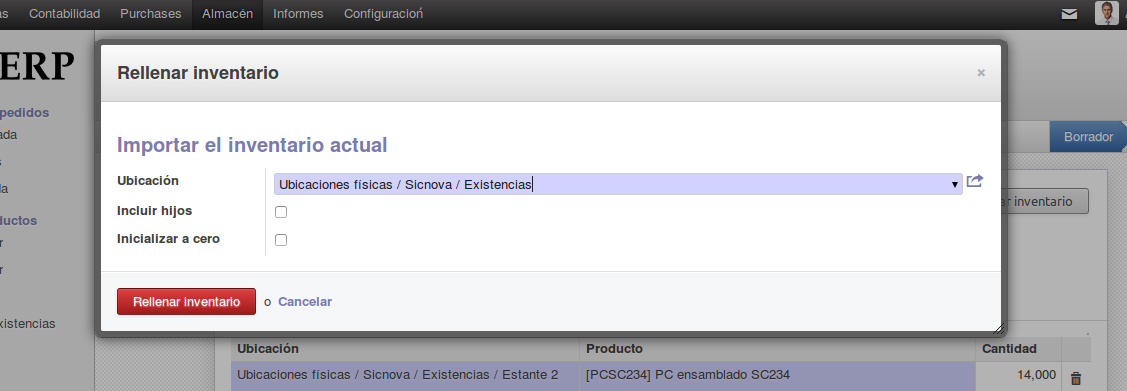
\includegraphics[width=\textwidth]{almacen/img/inv_imp.png}
\caption{Importación del inventario}
\label{ub:inventarioimportar}
\end{figure}


La otra pestaña disponible es la de \textbf{Inventario enviado}. En esta pestaña se rellena con la información de las transacciones de productos
ya realizadas, es decir, con la información de los albaranes de entrada salida. Mediante el botón \emph{Agregar}, que se puede apreciar en la
figura \ref{ub:inventarioenviado}, se despliega un menú que permite seleccionar que transacciones se van a incluir en esta pestaña. Lo habitual es
incluirlas todas.

\begin{figure}[H]
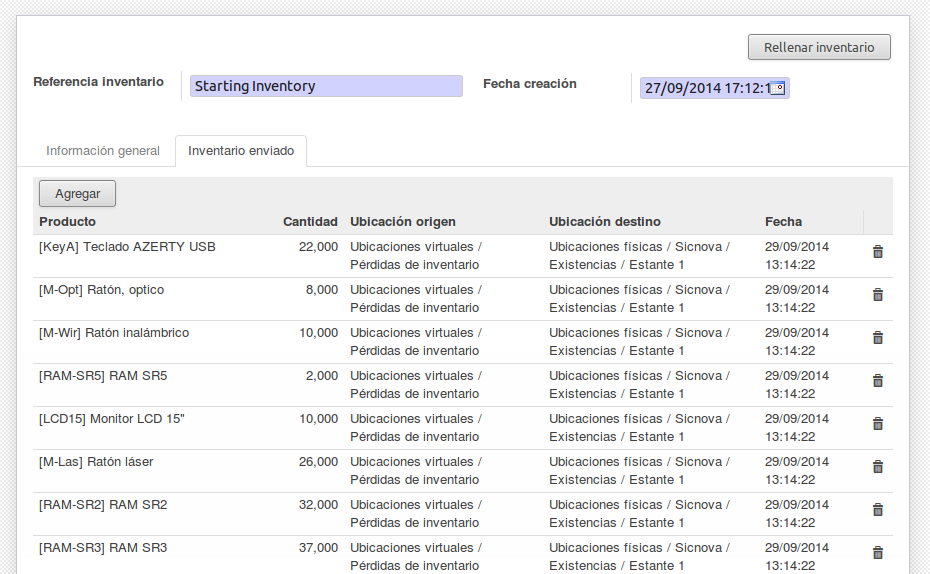
\includegraphics[width=\textwidth]{almacen/img/inv_env.png}
\caption{Importación del inventario}
\label{ub:inventarioenviado}
\end{figure}

Mediante el inventario físico se está indicando al software cuál es la cantidad de productos disponibles, y será la utilizada en el stock.
Con el inventario enviado el software calcula cuál sería la cantidad de productos disponibles en función del inventario existente anteriormente.
Si los calculos no corresponden, el software presentará esa diferencia en la ubicación \emph{Perdidas de inventario} como señal de la necesidad
de revisar las transacciones del producto correspondiente.




\section{Planificaciones}
Con OpenERP se pueden realizar planificaciones de aprovisionamiento. Se pueden definir unas reglas para poder tener siempre entre un mínimo y
un máximo de stock de productos. Esta configuración se realiza de manera individual para cada producto.

\subsection{Ejecutar planificadores}
Esta opción disparará todas las reglas de planificación de stock. En caso de que haya productos que no cumplas con las reglas del mínimo
establecido, generará automáticamente ordenes de abastecimiento que podrán ser comprobadas a mano y, a su vez, generará presupuestos de compra
en el módulo de compras con los artículos que no cumplan los mínimos.

El encargado de compras podrá ver aparecer los nuevos presupuestos de compra con una referencia a la orden de abastecimiento, sabiendo así que
la compra a realizar aparece para cumplir las mínimas cantidades en el stock.

\begin{figure}[H]
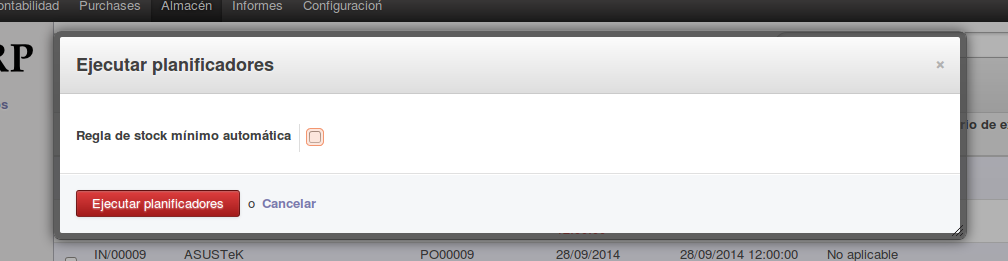
\includegraphics[width=\textwidth]{almacen/img/inv_plan.png}
\caption{Ejecución de planificadores}
\label{ub:inventarioplan}
\end{figure}

La figura \ref{ub:inventarioplan} muestra la ventana flotante que aparece tras seleccionar la opción de ejecución de los planificadores. Seleccionar
la opción \emph{Regla de stock mínima automática} hará que \textbf{todos} los productos que tengan un stock virtual menor que 0 ejecuten una orden
de abastecimiento para dejar este stock virtual a 0. No es recomendable utilizar esta opción puesto que puede generar pedidos indeseados.

\subsection{Excepciones abastecimiento}
Si tras ejecutar las planificaciones existiese algún problema con el stock, aparecerá aquí marcado en rojo. En cualquier otro caso se podrán ver como
en la figura \ref{ub:inventarioerr}

\begin{figure}[H]
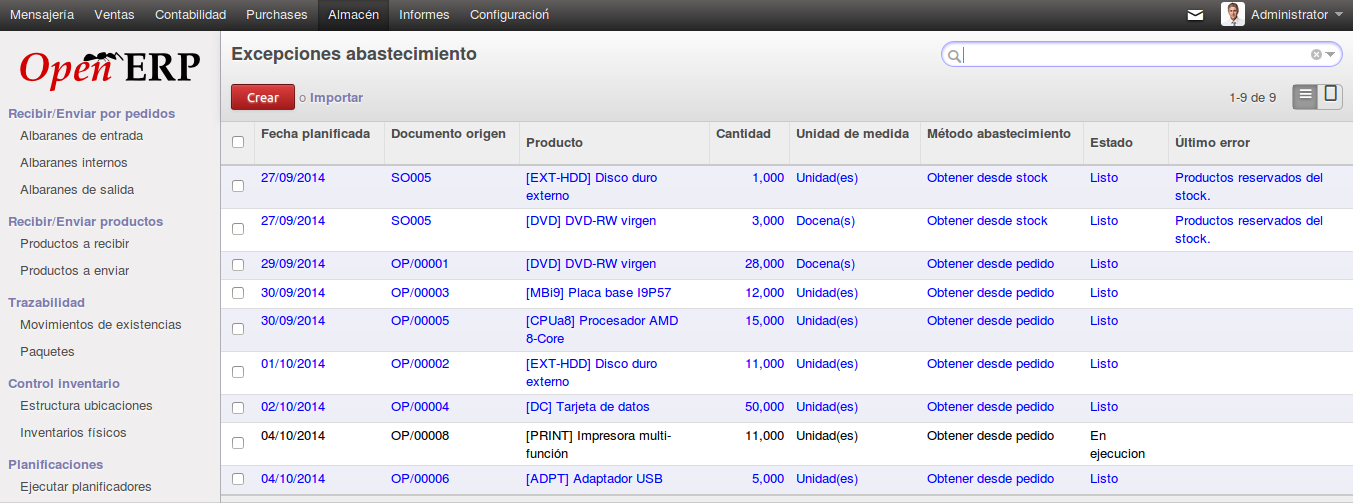
\includegraphics[width=\textwidth]{almacen/img/inv_error.png}
\caption{Ejecución de planificadores}
\label{ub:inventarioerr}
\end{figure}

Los campos que se pueden apreciar en esta sección son:

\begin{itemize}
  \item \textbf{Fecha planificada} -- Fecha calculada en la que se producirá el abastecimiento
  \item \textbf{Documento orgien} -- Referencia al documento que ha creado la orden de abastecimiento
  \item \textbf{Product} -- Producto al que hace referencia la orden
  \item \textbf{Cantidad} -- Cantidad de producto a pedir
  \item \textbf{Unidad de medida} -- Unidad de medida de las cantidades del producto
  \item \textbf{Método de abastecimiento} -- Indica de donde se obtiene el abastecimiento de este producto. Los que se puede encontrar es:
    \begin{itemize}
       \item[$\star$] \textbf{Obtener desde stock} - Las ordenes de venta, por ejemplo, pueden requerir de productos que estén en stock, en tal
                                                    caso, el abastecimiento del producto para el pedido se realiza desde el stock
       \item[$\star$] \textbf{Obtener desde pedido} - Algunos productos pueden configurarse para que cuando sean requeridos, se genere una orden 
                                                    de pedido. Cuando se ejecutan los planificadores, al encontrar productos que no cumplen los
                                                    mínimos también crea presupuestos para pedidos a proveedores, siendo pues este tipo de
                                                    abastecimiento también.
    \end{itemize}
  \item \textbf{Estado} -- Estado de la orden de excepción
    \begin{itemize}
      \item[$\star$] \textbf{Borrador} - Estado por defecto al crear la orden de abastecimiento. Si son creadas automáticamente, pasarán a alguno
                                         de los estados siguientes
      \item[$\star$] \textbf{Confirmado} - Estado alcanzado cuando se confirma el abastecimiento
      \item[$\star$] \textbf{En ejecución} - Estado tras la confirmación
      \item[$\star$] \textbf{Excepción} - Este estado se alcanza en el caso de que ocurra algún error. La orden aparecerá en rojo.
      \item[$\star$] \textbf{Listo} - Tras eliminar la excepción la orden pasará a este estado.
      \item[$\star$] \textbf{Esperando} - La orden está a la espera de que alguna otra sea atendida. Este estado puede aparecer si se usan opciones
                                          de manufacturación
    \end{itemize}
  \item \textbf{Último error} -- Especifica que es lo que ha provocado la excepción de abastecimiento de manera que permita buscar una solución.
\end{itemize}

\section{Reglas de reabastecimiento -- TODO}
\label{alm:reabastecimiento}
